% Generated by make_figures.py from traffic_tb.vcd (T2) - do not edit.
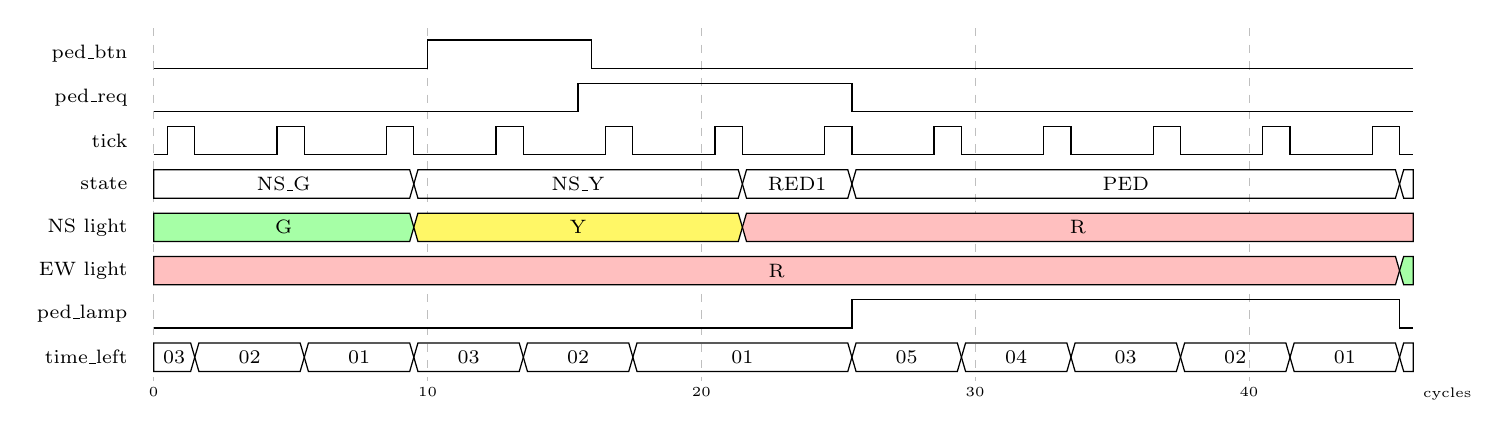
\begin{tikzpicture}[x=0.03478cm,y=1cm,font=\scriptsize,line width=0.45pt]
\draw[black!25,dashed,line width=0.3pt] (0.0,0.15) -- (0.0,-4.33);
\node[below=-1pt,font=\tiny] at (0.0,-4.33) {0};
\draw[black!25,dashed,line width=0.3pt] (100.0,0.15) -- (100.0,-4.33);
\node[below=-1pt,font=\tiny] at (100.0,-4.33) {10};
\draw[black!25,dashed,line width=0.3pt] (200.0,0.15) -- (200.0,-4.33);
\node[below=-1pt,font=\tiny] at (200.0,-4.33) {20};
\draw[black!25,dashed,line width=0.3pt] (300.0,0.15) -- (300.0,-4.33);
\node[below=-1pt,font=\tiny] at (300.0,-4.33) {30};
\draw[black!25,dashed,line width=0.3pt] (400.0,0.15) -- (400.0,-4.33);
\node[below=-1pt,font=\tiny] at (400.0,-4.33) {40};
\node[below=-1pt,font=\tiny,anchor=north west] at (460.0,-4.33) {cycles};
\node[anchor=east] at (-6,-0.18) {\code{ped\_btn}};
\draw (0.00,-0.36) -- (100.00,-0.36) -- (100.00,0.00) -- (160.00,0.00) -- (160.00,-0.36) -- (460.00,-0.36);
\node[anchor=east] at (-6,-0.73) {\code{ped\_req}};
\draw (0.00,-0.91) -- (155.00,-0.91) -- (155.00,-0.55) -- (255.00,-0.55) -- (255.00,-0.91) -- (460.00,-0.91);
\node[anchor=east] at (-6,-1.28) {\code{tick}};
\draw (0.00,-1.46) -- (5.00,-1.46) -- (5.00,-1.10) -- (15.00,-1.10) -- (15.00,-1.46) -- (45.00,-1.46) -- (45.00,-1.10) -- (55.00,-1.10) -- (55.00,-1.46) -- (85.00,-1.46) -- (85.00,-1.10) -- (95.00,-1.10) -- (95.00,-1.46) -- (125.00,-1.46) -- (125.00,-1.10) -- (135.00,-1.10) -- (135.00,-1.46) -- (165.00,-1.46) -- (165.00,-1.10) -- (175.00,-1.10) -- (175.00,-1.46) -- (205.00,-1.46) -- (205.00,-1.10) -- (215.00,-1.10) -- (215.00,-1.46) -- (245.00,-1.46) -- (245.00,-1.10) -- (255.00,-1.10) -- (255.00,-1.46) -- (285.00,-1.46) -- (285.00,-1.10) -- (295.00,-1.10) -- (295.00,-1.46) -- (325.00,-1.46) -- (325.00,-1.10) -- (335.00,-1.10) -- (335.00,-1.46) -- (365.00,-1.46) -- (365.00,-1.10) -- (375.00,-1.10) -- (375.00,-1.46) -- (405.00,-1.46) -- (405.00,-1.10) -- (415.00,-1.10) -- (415.00,-1.46) -- (445.00,-1.46) -- (445.00,-1.10) -- (455.00,-1.10) -- (455.00,-1.46) -- (460.00,-1.46);
\node[anchor=east] at (-6,-1.83) {state};
\draw[] (0.00,-1.83) -- (0.00,-1.65) -- (93.50,-1.65) -- (95.00,-1.83) -- (93.50,-2.01) -- (0.00,-2.01) -- cycle;
\node at (47.50,-1.83) {\code{NS\_G}};
\draw[] (95.00,-1.83) -- (96.50,-1.65) -- (213.50,-1.65) -- (215.00,-1.83) -- (213.50,-2.01) -- (96.50,-2.01) -- cycle;
\node at (155.00,-1.83) {\code{NS\_Y}};
\draw[] (215.00,-1.83) -- (216.50,-1.65) -- (253.50,-1.65) -- (255.00,-1.83) -- (253.50,-2.01) -- (216.50,-2.01) -- cycle;
\node at (235.00,-1.83) {\code{RED1}};
\draw[] (255.00,-1.83) -- (256.50,-1.65) -- (453.50,-1.65) -- (455.00,-1.83) -- (453.50,-2.01) -- (256.50,-2.01) -- cycle;
\node at (355.00,-1.83) {\code{PED}};
\draw[] (455.00,-1.83) -- (456.50,-1.65) -- (460.00,-1.65) -- (460.00,-1.83) -- (460.00,-2.01) -- (456.50,-2.01) -- cycle;
\node[anchor=east] at (-6,-2.38) {NS light};
\draw[fill=green!35] (0.00,-2.38) -- (0.00,-2.20) -- (93.50,-2.20) -- (95.00,-2.38) -- (93.50,-2.56) -- (0.00,-2.56) -- cycle;
\node at (47.50,-2.38) {\code{G}};
\draw[fill=yellow!60] (95.00,-2.38) -- (96.50,-2.20) -- (213.50,-2.20) -- (215.00,-2.38) -- (213.50,-2.56) -- (96.50,-2.56) -- cycle;
\node at (155.00,-2.38) {\code{Y}};
\draw[fill=red!25] (215.00,-2.38) -- (216.50,-2.20) -- (460.00,-2.20) -- (460.00,-2.38) -- (460.00,-2.56) -- (216.50,-2.56) -- cycle;
\node at (337.50,-2.38) {\code{R}};
\node[anchor=east] at (-6,-2.93) {EW light};
\draw[fill=red!25] (0.00,-2.93) -- (0.00,-2.75) -- (453.50,-2.75) -- (455.00,-2.93) -- (453.50,-3.11) -- (0.00,-3.11) -- cycle;
\node at (227.50,-2.93) {\code{R}};
\draw[fill=green!35] (455.00,-2.93) -- (456.50,-2.75) -- (460.00,-2.75) -- (460.00,-2.93) -- (460.00,-3.11) -- (456.50,-3.11) -- cycle;
\node[anchor=east] at (-6,-3.48) {\code{ped\_lamp}};
\draw (0.00,-3.66) -- (255.00,-3.66) -- (255.00,-3.30) -- (455.00,-3.30) -- (455.00,-3.66) -- (460.00,-3.66);
\node[anchor=east] at (-6,-4.03) {\code{time\_left}};
\draw[] (0.00,-4.03) -- (0.00,-3.85) -- (13.50,-3.85) -- (15.00,-4.03) -- (13.50,-4.21) -- (0.00,-4.21) -- cycle;
\node at (7.50,-4.03) {\code{03}};
\draw[] (15.00,-4.03) -- (16.50,-3.85) -- (53.50,-3.85) -- (55.00,-4.03) -- (53.50,-4.21) -- (16.50,-4.21) -- cycle;
\node at (35.00,-4.03) {\code{02}};
\draw[] (55.00,-4.03) -- (56.50,-3.85) -- (93.50,-3.85) -- (95.00,-4.03) -- (93.50,-4.21) -- (56.50,-4.21) -- cycle;
\node at (75.00,-4.03) {\code{01}};
\draw[] (95.00,-4.03) -- (96.50,-3.85) -- (133.50,-3.85) -- (135.00,-4.03) -- (133.50,-4.21) -- (96.50,-4.21) -- cycle;
\node at (115.00,-4.03) {\code{03}};
\draw[] (135.00,-4.03) -- (136.50,-3.85) -- (173.50,-3.85) -- (175.00,-4.03) -- (173.50,-4.21) -- (136.50,-4.21) -- cycle;
\node at (155.00,-4.03) {\code{02}};
\draw[] (175.00,-4.03) -- (176.50,-3.85) -- (253.50,-3.85) -- (255.00,-4.03) -- (253.50,-4.21) -- (176.50,-4.21) -- cycle;
\node at (215.00,-4.03) {\code{01}};
\draw[] (255.00,-4.03) -- (256.50,-3.85) -- (293.50,-3.85) -- (295.00,-4.03) -- (293.50,-4.21) -- (256.50,-4.21) -- cycle;
\node at (275.00,-4.03) {\code{05}};
\draw[] (295.00,-4.03) -- (296.50,-3.85) -- (333.50,-3.85) -- (335.00,-4.03) -- (333.50,-4.21) -- (296.50,-4.21) -- cycle;
\node at (315.00,-4.03) {\code{04}};
\draw[] (335.00,-4.03) -- (336.50,-3.85) -- (373.50,-3.85) -- (375.00,-4.03) -- (373.50,-4.21) -- (336.50,-4.21) -- cycle;
\node at (355.00,-4.03) {\code{03}};
\draw[] (375.00,-4.03) -- (376.50,-3.85) -- (413.50,-3.85) -- (415.00,-4.03) -- (413.50,-4.21) -- (376.50,-4.21) -- cycle;
\node at (395.00,-4.03) {\code{02}};
\draw[] (415.00,-4.03) -- (416.50,-3.85) -- (453.50,-3.85) -- (455.00,-4.03) -- (453.50,-4.21) -- (416.50,-4.21) -- cycle;
\node at (435.00,-4.03) {\code{01}};
\draw[] (455.00,-4.03) -- (456.50,-3.85) -- (460.00,-3.85) -- (460.00,-4.03) -- (460.00,-4.21) -- (456.50,-4.21) -- cycle;
\end{tikzpicture}
